\documentclass[12pt]{article}
\usepackage{fontspec}
\usepackage{babel}[russian]

\setmainfont{Times New Roman}

\usepackage{rotating}

\usepackage{graphicx}   % Пакет для включения рисунков
\DeclareGraphicsExtensions{.jpg,.pdf,.png}
% С такими оно полями оно работает по-умолчанию:
\RequirePackage[left=10mm,right=10mm,top=10mm,bottom=20mm]{geometry}

\linespread{1}

\usepackage{fancyhdr}
\fancyhf{}
\fancyhead[C]{\thepage\\RU.17701729.04.01-01 ТЗ 01-1}
\renewcommand{\headrulewidth}{0pt}

\fancyfoot[C]{\small \begin{tabular}{l}
	\end{tabular}\\ \begin{tabular}{|l|l|l|l|l|}
		\hline
		\multicolumn{1}{|c|}{} &              &              &              &              \\ \hline
		Изм.                   & Лист         & № докум.     & Подп.        & Дата         \\ \hline
		RU.17701729.04.01-01 ТЗ 01-1                 &              &              &              &              \\ \hline
		Инв. № подл.           & Подп. и дата & Взам. инв. № & Инв. № дубл. & Подп. и дата \\ \hline
\end{tabular}}
\renewcommand{\headrulewidth}{0pt}



\usepackage{indentfirst} % Красная строка после заголовка
\setlength\parindent{1.25cm} 

\usepackage{sectsty}
\sectionfont{\fontsize{14}{15}\selectfont}

\AtBeginDocument{\addtocontents{toc}{\protect\thispagestyle{fancy}}} 

\usepackage{multirow}

\usepackage{afterpage}

\usepackage{lipsum}
\setlength{\parindent}{5ex}

\usepackage{titlesec}
\titleformat*{\section}{\centering\large\bfseries}
\titleformat*{\subsection}{\normalsize\bfseries}

\usepackage{enumerate}

\begin{document}
	\pagestyle{empty}
	%\newgeometry{left=30mm}
%\afterpage{\restoregeometry}

\begin{center} 

		\textbf{ПРАВИТЕЛЬСТВО РОССИЙСКОЙ ФЕДЕРАЦИИ}\\
		\textbf{НАЦИОНАЛЬНЫЙ ИССЛЕДОВАТЕЛЬСИКИЙ УНИВЕРСИТЕТ}\\
		\textbf{ВЫСШАЯ ШКОЛА ЭКОНОМИКИ}\\
		\bigskip
		Факультет компьютерных наук\\
		Департамент программной инженерии\\
		\bigskip
		\bigskip
		\begin{table}[h]
			\centering
			\begin{tabular}{c p{10mm} c}
				\begin{tabular}[c]{@{}c@{}}СОГЛАСОВАНО\\ Старший преподаватель\\ департамента программной инженерии\\
					факультета компьютерных наук\bigskip\bigskip\bigskip\end{tabular}                     && \begin{tabular}[c]{@{}c@{}}УТВЕРЖДАЮ\\ Академический руководитель\\ образовательной программы\\ «Программная инженерия»\\ профессор департамента программной\\ инженерии, канд. техн. наук\bigskip\end{tabular} \\
				\begin{tabular}[c]{@{}c@{}}\_\_\_\_\_\_\_\_\_\_\_\_\_\_\_\_\_\_М.К. Горденко\\ «\_\_\_» \_\_\_\_\_\_\_\_\_\_\_\_\_ 2019 г.\end{tabular} && \begin{tabular}[c]{@{}c@{}}\_\_\_\_\_\_\_\_\_\_\_\_\_\_\_\_\_\_В.В. Шилов\\ «\_\_\_» \_\_\_\_\_\_\_\_\_\_\_\_\_ 2019 г.\end{tabular}                                                                   
			\end{tabular}
		\end{table}
		
	
		\begin{table}[h]
			\begin{tabular}[t]{cc}
				\small
				\begin{tabular}{|c|c|}
					\hline
					\begin{sideways}
						\textit{\textbf{$\;$Подп. и дата$\;$}}
					\end{sideways} &  \\ \hline
					\begin{sideways}\textit{\textbf{$\;$Инв. № дубл.$\;$}}\end{sideways} &  \\ \hline
					\begin{sideways}\textit{\textbf{$\;$Взам. инв. №$\;$}}\end{sideways} &  \\ \hline
					\begin{sideways}\textit{\textbf{$\;$Подп. и дата$\;$}}\end{sideways} &  \\ \hline
					\begin{sideways}\textit{\textbf{$\;$Инв. № подл$\;$}}\end{sideways}  &  \\ \hline
				\end{tabular}
			& \begin{tabular}{c}
				{\Large \textbf{МОБИЛЬНОЕ ПРИЛОЖЕНИЕ <<АРТ-КВЕСТ>>}}\\

				\\
				\\
				\large \textbf{Техническое задание}\\
				\\
				\textbf{ЛИСТ УТВЕРЖДЕНИЯ}\\
				\\
				\textbf{RU.17701729.04.01-01 ТЗ 01-1-ЛУ}\\		
				\\				
				\\				
				\\
				\\		
		 		\begin{tabular}{p{85mm} c}
		 			& \begin{tabular}[c]{@{}c@{}}Исполнитель\\ студент группы \_\_\_\_\_\_\_\_\_\\ \_\_\_\_\_\_\_\_\_\_\_\_\_\_\_\_\_\_\_\_\_XXXXXXXXXX\\ «\_\_\_\_»\_\_\_\_\_\_\_\_\_\_\_\_\_\_\_\_\_\_\_\_\_\_\_2019 г.\end{tabular}
		 		\end{tabular}
			
				\\
				\\
				\\
				\\
				\\
				\\
				\\
				\\
			
				
			\end{tabular}
			
			\end{tabular}
		\end{table}
		





\end{center} 


\vfill 


\centering \large \textbf{Москва 2019}

\thispagestyle{empty}


	\begin{flushleft}
	
	\qquad \qquad\begin{tabular}{l}
		\large УТВЕРЖДЁН\\
		\textbf{RU.17701729.02.02-01 ТЗ 01-1-ЛУ}
	\end{tabular}
\end{flushleft}


	\bigskip
	\bigskip
	\bigskip
	\bigskip
	\bigskip
	\bigskip
	\bigskip
	\bigskip
	\bigskip
	\bigskip
	\bigskip
	\bigskip
	\bigskip
	\bigskip
	\bigskip
	\bigskip
	\bigskip 
	\bigskip
	
\begin{table}[h]
	\begin{tabular}[t]{cc}
		\small
		\begin{tabular}{|c|c|}
			\hline
			\begin{sideways}
				\textit{\textbf{$\;$Подп. и дата$\;$}}
			\end{sideways} &  \\ \hline
			\begin{sideways}\textit{\textbf{$\;$Инв. № дубл.$\;$}}\end{sideways} &  \\ \hline
			\begin{sideways}\textit{\textbf{$\;$Взам. инв. №$\;$}}\end{sideways} &  \\ \hline
			\begin{sideways}\textit{\textbf{$\;$Подп. и дата$\;$}}\end{sideways} &  \\ \hline
			\begin{sideways}\textit{\textbf{$\;$Инв. № подл$\;$}}\end{sideways}  &  \\ \hline
		\end{tabular}
		& \begin{tabular}{p{5mm} c} &
			\begin{tabular}{c}
				
				\textbf{{\Large МОБИЛЬНОЕ ПРИЛОЖЕНИЕ <<АРТ-КВЕСТ>>}}\\
				\\
				
				\\
				
				\large \textbf{Техническое задание}\\
				\\
				\textbf{RU.17701729.04.01-01 ТЗ 01-1-ЛУ}\\		
				\\				
				\textbf{Листов 20}				
				\\
				\\		
				
				
				\\
				\\
				\\
				\\
				\\
				\\
				\\
				\\
				\\
				\\
				\\
				
			\end{tabular}
			
			
			
		\end{tabular}
		
	\end{tabular}
\end{table}

\vfill

\textbf{\large Москва 2019}

\thispagestyle{empty}
	\newgeometry{top=20mm, left=20mm,right=20mm,bottom=40mm}
	\afterpage{\restoregeometry}
	\setcounter{page}{2}
	\footnotesize
	\def\contentsname{\textbf{ОГЛАВЛЕНИЕ}}
    \tableofcontents
	\flushleft
	\normalsize
	\pagestyle{fancy}


\section{ВВЕДЕНИЕ}


\subsection{Наименование программы} 
	
\subsubsection{Наименование программы на русском языке}
	
\hspace{10mm}	Мобильное приложение <<Арт-квест>>.
	
\subsubsection{Наименование программы на английском языке}	
	
	\hspace{10mm} Mobile application <<Art-quest>>.
	
\subsection{Краткая характеристика области применения программы}
	
	
\hspace{10mm} Людям скучно ходить в музеи из-за сухой подачи информации и нехватки знаний. Приложение «Арт-квест» поможет не заскучать на выставке и провести время увлекательно как одному, так и в компании друзей. Все, что нужно делать — проходить задания, за которые в дальнейшем вы сможете приобрести награды.

\hspace{10mm} Разрабатываемая программа должна привлечь людей к выставкам и показать, что искусство -- это интересно.
	\pagestyle{fancy}

\section{ОСНОВАНИЯ ДЛЯ РАЗРАБОТКИ}


\subsection{Документы, на основании которых ведется разработка} 
	
\hspace{10mm} Приказ декана факультета компьютерных наук Национального Исследовательского Университета "Высшая школа экономики" XXXXXXXXXX
	
\subsection{Наименование темы разработки}

\hspace{10mm} Наименование программы -- мобильное приложение <<Арт-квест>> (mobile application <<Art-quest>>).

\hspace{10mm} Программа выполняется в рамках темы проектной работы в соответствии с учебным
планом подготовки бакалавров по направлению 09.03.04 «Программная инженерия»
Национального исследовательского университета «Высшая школа экономики», факультет компьютерных наук в рамках предмета <<Групповая динамика и коммуникации в программной инженерии>>.
	


	\pagestyle{fancy}


\section{НАЗНАЧЕНИЕ РАЗРАБОТКИ}


\subsection{Функциональное назначение} 
	
\hspace{10mm} Пользователи программы могут не только ознакомиться с проходящими арт-выставками по различным категориям искусства и узнать основную информацию о них, но и пройти квесты по посещенным выставкам и музеям, получив ценные призы. Приложение предоставляет пользователям личную страницу, где они смогут разместить информацию о своей культурной жизни. Кроме того в приложении можно купить билеты на мероприятия он-лайн.
	
\subsection{Эксплуатационное назначение}

\hspace{10mm} <<Арт-квест>> поможет любителям арт-выставок и музеев узнавать новую информацию о текущих мероприятиях и удобно приобретать на них билеты. Кроме того, приложение будет интересно людям, которые только открывают для себя мир искусства. Данная программа послужит для них дополнительной мотивацией в посещении арт-объектов и подтолкнет к изучению новой информации.

\hspace{10mm} Таким образом, программный продукт будет интересен людям любых интересов.

	\pagestyle{fancy}

\begin{center}
		\section{ТРЕБОВАНИЯ К ПРОГРАММЕ}
\end{center}	

\subsection{Требования к функциональным характеристикам} 
	
	\subsubsection{Требования к составу выполняемых функций}	

		\hspace{10mm} Программа выполняется в рамках темы курсовой работы в соответствии с учебным
		планом подготовки бакалавров по направлению 09.03.04 «Программная инженерия»
		Национального исследовательского университета «Высшая школа экономики», факультет компьютерных наук.
		
		\hspace{10mm} Разработка требований велась совместно с командой и заказчиком в рамках предмета «Групповая динамика и коммуникации в программной инженерии»
		
		\textit{Состав команды:}
		\begin{itemize}
			\item Борис Малашенко -- android-developer;
			\item Тимофей Семенкович -- backend-developer;
			\item Дмитрий Сорокин -- iOS-developer;
			\item Дмитрий Штеменко -- android-developer;
		\end{itemize}
		
		\textit{Заказчик:}
		\begin{itemize}
			\item Авшалумова Бациин, Школа дизайна/ Кафедра «Коммуникационный дизайн».
		\end{itemize}

	\subsection*{FR-1. Авторизация клиента}

	\hspace{10mm}Чтобы использовать все возможности программы, клиент должен авторизоваться в системе
	
		\subsubsection*{FR-1.1.} При регистрации в программе  клиенту необходимо заполнить обязательные поля регистрации:
		
		\begin{enumerate}
			\item
				имя и фамилия;
			\item
				email или номер телефона;
			\item
				пароль.	
				
		\end{enumerate}
	
		\subsubsection*{FR-1.2.} 
		\hspace{10mm} Уже зарегистрированный клиент для входа в социальную сеть должен ввести
		свою почту или номер телефона и пароль.
	
		\subsubsection*{FR-1.3.}
		\hspace{10mm}После успешной регистрации пользователю будет выслан код
		на введенную им почту, который нужно ввести в специальное поле в приложении, только после правильного ввода кода клиент сможет войти в социальную
		сеть.

		\subsubsection*{FR-1.4.}
		\hspace{10mm} Если пользователь забыл пароль от системы, ему на почту/телефона должна быть выслана форма восстановления.
		
		\subsubsection*{FR-1.5.}
		\hspace{10mm} У пользователя должна быть возможность авторизоваться при помощи:
		\begin{enumerate}
			\item социальной сети Facebook;
			\item социальной сети Twitter;
			\item социальной сети Вконтакте.
		\end{enumerate}
		
		\subsection*{FR-2. Прохождение квестов}
		
		\subsubsection*{FR-2.1.}

		
		\hspace{10mm}У пользователя должна быть возможность просмотра актуальных квестов с основной информацией о них.
		
		\subsubsection*{FR-2.2.}
		
		
		\hspace{10mm}Должна быть возможность фильтровать список квестов по параметрам:
		
		\begin{enumerate}
			\item последние / популярные;
			\item сложность;		
			\item тема;	
			\item дистанция от пользователя до места проведения квеста;
			\item примерное время, за которое проходится выставка, связанная с квестом.
		\end{enumerate}
	
		\subsubsection*{FR-2.3.}
		
		\hspace{10mm} При выборе квеста пользователю должна быть предоставлена основная информация о квесте и выставке, связанной с ним. Должны отображаться следующие данные:
		\begin{enumerate}
		 	\item краткая информация о мероприятии;
		 	\item цена билета на мероприятие;
		 	\item возраст, с которого позволен вход на мероприятие;
		 	\item время прохождения мероприятия;
		 	\item сложность мероприятия;
		 	\item отзывы о мероприятии.
		\end{enumerate}
	
		\hspace{10mm} Если пользователь посещал связанную с квестом выставку, у него должна быть возможность пройти этот квест.
		
		\subsubsection*{FR-2.4.}
		
			\hspace{10mm} При прохождении вопросов квеста пользователь может использовать подсказку на данный вопрос, но потеряет часть своих баллов при верном ответе.
			
			\hspace{10mm} Пользователю должны предоставляться как минимум три вида вопросов:
			\begin{enumerate}
				\item с выбором ответа из списка;
				\item вида "собери картинку";
				\item вида "впиши верное слово".
			\end{enumerate}
		
		\subsubsection*{FR-2.5.}
		
			\hspace{10mm} После прохождения квеста у пользователя должна быть возможность оценить пройденный квест.
		
			\hspace{10mm} Кроме того пользователь сможет разместить запись о прохождении и оценке на личной странице приложения <<Арт-квест>>, либо на странице одной из своих социальных сетей.
			
		\subsubsection*{FR-2.6.}
		
			\hspace{10mm} При успешном прохождении квеста, пользователь должен получить бонусные баллы
			
			
	\subsection*{FR-3. Профиль}
	
			\hspace{10mm} У пользователя должна быть личная страница с основной информацией:
			\begin{enumerate}
				\item имя и фамилия пользователя
				\item пройденные квесты;
				\item количество баллов.
			\end{enumerate}
		
	\subsection*{FR-4. Таблицы лидеров}
	
			\hspace{10mm} В приложении должны быть таблицы лидеров за:
			\begin{enumerate}
				\item все время;
				\item последний месяц;
				\item последнюю неделю.
			\end{enumerate}
		
		\hspace{10mm} Пользователь должен видеть свое положение в каждой из таблиц.
		
	\subsection*{FR-5. Магазин наград}
	
		\hspace{10mm} Пользователь должен видеть все товары, которые он может приобрести за баллы.
		
	\subsection*{FR-6. Настройки}	
	
		\hspace{10mm} У пользователя должна быть возможность изменить свои:
		\begin{enumerate}
			\item фото;
			\item имя и фамилию;
			\item пароль;
			\item электронную почту;
			\item телефон.
		\end{enumerate}
	
		\hspace{10mm} У клиента должна быть возможность включить/выключить уведомления, звуковые эффекты.
		
		\hspace{10mm} Должна быть возможность поделиться успехами, если привязаны соц. сети, оставить отзыв программе, либо выйти из аккаунта.
	\pagestyle{fancy}



	\section{ТРЕБОВАНИЯ К ПРОГРАММНОЙ ДОКУМЕНТАЦИИ}


\subsection{Предварительный состав программной документации} 
	
\normalsize
\begin{enumerate}
	\item <<Мобильное приложение <<Арт-квест>>. Техническое задание (ГОСТ 19.201-78);
	\item <<Мобильное приложение <<Арт-квест>>. Программа и методика испытаний (ГОСТ 19.301-78);
	\item <<Мобильное приложение <<Арт-квест>>. Текст программы (ГОСТ 19.401-78);
	\item <<Мобильное приложение <<Арт-квест>>. Пояснительная записка (ГОСТ 19.404-79);
	\item <<Мобильное приложение <<Арт-квест>>. Руководство оператора (ГОСТ 19.505-79); 
\end{enumerate}
	
\subsection{Специальные требования к программной документации}

	\begin{enumerate}
		\item Все документы к программе должны быть выполнены в соответствии с ГОСТ 19.106-78 [2] и ГОСТ к этому виду документа (см. п. 5.1.).
		\item Пояснительная записка должна быть загружена в систему Антиплагиат через ЛМС НИУ ВШЭ. Лист, подтверждающий загрузку пояснительной записки, сдается в учебный офис вместе со всеми материалами не позже, чем за день до защиты проектной работы.
		\item Вся документация сдается в печатном виде, при этом она должна быть обязательно подписана академическим руководителем образовательной программы 09.03.04 «Программная инженерия», руководителем разработки и исполнителем перед сдачей проектной работы в учебный офис не позже одного дня до защиты.
		\item Вся документация и программа также сдается в электронном виде в формате .pdf или .docx. в архиве формата .rar или .zip..
	\end{enumerate}
	


	\pagestyle{fancy}

\normalsize


\section{ТЕХНИКО-ЭКОНОМИЧЕСКИЕ ПОКАЗАТЕЛИ}

\subsection{Предполагаемая потребность}	
	
\hspace{10mm} <<Арт-квест>> поможет любителям арт-выставок и музеев узнавать новую информацию о текущих мероприятиях и удобно приобретать на них билеты. Кроме того, приложение будет интересно людям, которые только открывают для себя мир искусства. Данная программа послужит для них дополнительной мотивацией в посещении арт-объектов и подтолкнет к изучению новой информации.

\hspace{10mm} Таким образом, программный продукт будет интересен людям любых интересов.
	
\subsection{Ориентировочная экономическая эффективность}
	
\hspace{10mm}В данной таблице приведен список прямых и косвенных конкурентов социальной сети.

\begin{table}[h]
	\caption{Виды конкурентов}
	\centering
	\begin{tabular}{|l|l|l|}
		\hline
		\textbf{Название}                      & \textbf{Описание}                                                                                            & \textbf{Вид} \\ \hline
		\textit{КудаГо}                        & \begin{tabular}[c]{@{}l@{}}Сайт с информацией о многих\\ мероприятиях крупных городов\\ России\end{tabular}  & Прямой       \\ \hline
		\textit{Музей Эрмитаж}                 & Приложение Эрмитажа                                                                                          & Косвенный    \\ \hline
		\textit{Second Canvas Museo del Prado} & \begin{tabular}[c]{@{}l@{}}Приложение для изучения\\ живописи\end{tabular}                                   & Косвенный    \\ \hline
		\textit{MoMA}                          & \begin{tabular}[c]{@{}l@{}}Приложение музея современного\\ искусства в Нью-Йорке.\end{tabular}               & Косвенный    \\ \hline
		\textit{Guggenheim}                    & \begin{tabular}[c]{@{}l@{}}Приложение музея\\ Соломона Гуггенхайма\end{tabular}                              & Косвенный    \\ \hline
		\textit{Musée du Louvre HD}            & Приложение Лувра                                                                                             & Косвенный    \\ \hline
		\textit{Your Art}                      & \begin{tabular}[c]{@{}l@{}}Цифровая версия\\ Национальной галереи\\ искусства в Вашингтоне\end{tabular}      & Косвенный    \\ \hline
		\textit{Love Art: National Gallery}    & \begin{tabular}[c]{@{}l@{}}В приложении содержится\\ информация о западноевропейской\\ живописи\end{tabular} & Косвенный    \\ \hline
		\textit{Приложения Артхив}             & \begin{tabular}[c]{@{}l@{}}Набор приложений о различных\\ художниках\end{tabular}                            & Косвенный    \\ \hline
	\end{tabular}
\end{table}

 \hspace{10mm} Большая часть аналогов данного приложения привязаны к одному музею, либо художнику и не имеют игровой составляющей.

\hspace{10mm} Таким образом, мобильное приложение <<Арт-квест>> будет пользоваться спросом из-за малого числа прямых конкурентов.

\hspace{10mm} Ниже приведена таблица с детальным анализом конкурентов социальной сети. При
подсчете финальной оценки кажого конкурента большим приоритетом в формуле обладали показатели критериев «Личная страница пользователя», «Игровая составляющая» и «Информационная составляющая». Именно эти критерии наиболее релевантны для будущих пользователей разрабатываемого приложения.

\hspace{10mm} Для вычисления финальной оценки был применен следующий алгоритм: критерии
оценки были разбиты на следующие кластеры исходя из смысла.

\hspace{10mm} Финальная оценка рассчитывалась как среднее арифметическое всех оценок.

\begin{table}[h]
	\centering
	\caption{Детальный анализ конкурентов}
	\begin{tabular}{llllllllll}
		\hline
		\multicolumn{1}{|l|}{} & \multicolumn{1}{l|}{\begin{sideways}
				\textbf{КудаГо}\end{sideways}} & \multicolumn{1}{l|}{\textbf{\begin{sideways}Музей Эрмитаж\end{sideways}}} & \multicolumn{1}{l|}{\textbf{\begin{sideways}Second Canvas\end{sideways}} \textbf{\begin{sideways}
					$\;$
			\end{sideways}}
			\textbf{\begin{sideways}
					Museo del Prado
			\end{sideways}}} & \multicolumn{1}{l|}{\textbf{\begin{sideways}MoMA\end{sideways}}} & \multicolumn{1}{l|}{\textbf{\begin{sideways}Guggenheim\end{sideways}}} & \multicolumn{1}{l|}{\textbf{\begin{sideways}Musee du Louvre $\;$\end{sideways}}} & \multicolumn{1}{l|}{\textbf{\begin{sideways}Your Art\end{sideways}}} & \multicolumn{1}{l|}{\textbf{\begin{sideways}Love Art\end{sideways}}} & \multicolumn{1}{l|}{\textbf{\begin{sideways}Артхив\end{sideways}}} \\ \hline
		\multicolumn{1}{|l|}{\textbf{Личная страница пользователя}} & \multicolumn{1}{l|}{3} & \multicolumn{1}{l|}{3} & \multicolumn{1}{l|}{3} & \multicolumn{1}{l|}{4} & \multicolumn{1}{l|}{3} & \multicolumn{1}{l|}{5} & \multicolumn{1}{l|}{6} & \multicolumn{1}{l|}{3} & \multicolumn{1}{l|}{8} \\ \hline
		\multicolumn{1}{|l|}{\textbf{Топ участников}} & \multicolumn{1}{l|}{0} & \multicolumn{1}{l|}{0} & \multicolumn{1}{l|}{0} & \multicolumn{1}{l|}{0} & \multicolumn{1}{l|}{0} & \multicolumn{1}{l|}{0} & \multicolumn{1}{l|}{0} & \multicolumn{1}{l|}{0} & \multicolumn{1}{l|}{0} \\ \hline
		\multicolumn{1}{|l|}{\textbf{Игровая составляющая}} & \multicolumn{1}{l|}{0} & \multicolumn{1}{l|}{0} & \multicolumn{1}{l|}{0} & \multicolumn{1}{l|}{0} & \multicolumn{1}{l|}{0} & \multicolumn{1}{l|}{0} & \multicolumn{1}{l|}{0} & \multicolumn{1}{l|}{0} & \multicolumn{1}{l|}{0} \\ \hline
		\multicolumn{1}{|l|}{\textbf{Информационная составляющая}} & \multicolumn{1}{l|}{10} & \multicolumn{1}{l|}{5} & \multicolumn{1}{l|}{8} & \multicolumn{1}{l|}{7} & \multicolumn{1}{l|}{7} & \multicolumn{1}{l|}{6} & \multicolumn{1}{l|}{7} & \multicolumn{1}{l|}{8} & \multicolumn{1}{l|}{7} \\ \hline
		\multicolumn{1}{|l|}{\textbf{Покупка билетов онлайн}} & \multicolumn{1}{l|}{6} & \multicolumn{1}{l|}{9} & \multicolumn{1}{l|}{6} & \multicolumn{1}{l|}{9} & \multicolumn{1}{l|}{7} & \multicolumn{1}{l|}{9} & \multicolumn{1}{l|}{7} & \multicolumn{1}{l|}{4} & \multicolumn{1}{l|}{0} \\ \hline
		\multicolumn{1}{|l|}{\textbf{Внутренний магазин}} & \multicolumn{1}{l|}{2} & \multicolumn{1}{l|}{2} & \multicolumn{1}{l|}{8} & \multicolumn{1}{l|}{9} & \multicolumn{1}{l|}{9} & \multicolumn{1}{l|}{2} & \multicolumn{1}{l|}{8} & \multicolumn{1}{l|}{10} & \multicolumn{1}{l|}{2} \\ \hline
		\multicolumn{1}{|l|}{\textbf{Новостная лента}} & \multicolumn{1}{l|}{10} & \multicolumn{1}{l|}{5} & \multicolumn{1}{l|}{5} & \multicolumn{1}{l|}{6} & \multicolumn{1}{l|}{6} & \multicolumn{1}{l|}{8} & \multicolumn{1}{l|}{8} & \multicolumn{1}{l|}{6} & \multicolumn{1}{l|}{10} \\ \hline
		\multicolumn{1}{|l|}{\textbf{Интерфейс}} & \multicolumn{1}{l|}{5} & \multicolumn{1}{l|}{7} & \multicolumn{1}{l|}{5} & \multicolumn{1}{l|}{6} & \multicolumn{1}{l|}{6} & \multicolumn{1}{l|}{5} & \multicolumn{1}{l|}{4} & \multicolumn{1}{l|}{7} & \multicolumn{1}{l|}{2} \\ \hline
		\multicolumn{1}{|l|}{\textbf{Наличие десктопного приложения}} & \multicolumn{1}{l|}{0} & \multicolumn{1}{l|}{0} & \multicolumn{1}{l|}{0} & \multicolumn{1}{l|}{0} & \multicolumn{1}{l|}{0} & \multicolumn{1}{l|}{0} & \multicolumn{1}{l|}{0} & \multicolumn{1}{l|}{0} & \multicolumn{1}{l|}{0} \\ \hline
		\multicolumn{1}{|l|}{\textbf{Наличие ios / android версии}} & \multicolumn{1}{l|}{0} & \multicolumn{1}{l|}{10} & \multicolumn{1}{l|}{10} & \multicolumn{1}{l|}{0} & \multicolumn{1}{l|}{0} & \multicolumn{1}{l|}{0} & \multicolumn{1}{l|}{0} & \multicolumn{1}{l|}{0} & \multicolumn{1}{l|}{10} \\ \hline
		\multicolumn{1}{|l|}{\textbf{Наличие web приложения}} & \multicolumn{1}{l|}{10} & \multicolumn{1}{l|}{10} & \multicolumn{1}{l|}{10} & \multicolumn{1}{l|}{10} & \multicolumn{1}{l|}{10} & \multicolumn{1}{l|}{10} & \multicolumn{1}{l|}{10} & \multicolumn{1}{l|}{10} & \multicolumn{1}{l|}{10} \\ \hline
		& 4.18 & 4.64 & 5 & 4.64 & 4.36 & 4.09 & 4.55 & 4.36 & 4.45
	\end{tabular}
\end{table}

	\pagestyle{fancy}

\begin{center}
	\section{СТАДИИ И ЭТАПЫ РАЗРАБОТКИ}
\end{center}	
	
\subsection{Необходимые стадии разработки, этапы и содержание работ}

\begin{enumerate}[I.]
	\item Техническое задание: \textit{(ноябрь-декабрь, 2019)}
	\begin{enumerate}[1.]
		\item Этапы разработки: \textit{(ноябрь, 2019)}
		\begin{enumerate}[1.]
			\item обоснование необходимости разработки программы;
			\item постановка задачи;
			\item cбор исходных материалов;
			\item выбор и обоснование критериев эффективности и качества разрабатываемой программы;
			\item обоснование необходимости проведения научно-исследовательских работ;
		\end{enumerate}
	
		\item  Разработка и утверждение технического задания: \textit{(ноябрь-декабрь, 2019)}
		
		\begin{enumerate}[1.]
			\item определение требований к программе; \textit{(декабрь, 2019)}
			\item определение стадий, этапов и сроков разработки программы и документации на неё; \textit{(декабрь, 2019)}
			\item согласование и утверждение технического задания; \textit{(декабрь, 2019)}
		\end{enumerate}
	\end{enumerate}

	\item Проект \textit{(ноябрь – май, 2019/20)}
	
	\begin{enumerate}[1.]
		\item Начальная стадия разработки; \textit{(ноябрь, 2019)}
		
		\begin{enumerate}[1.]
			\item выбор темы;
			\item анализ предметной области;
			\item анализ конкурентов; (см. 6.2)
			\item SWOT-анализ; (см. 8.2)
			\item выявление требований;
			\item распределение ролей;
		\end{enumerate}
		
		\item Определение основного функционала; (декабрь, 2019)
		
		\item Дизайн; (ноябрь-декабрь, 2019)
		
		\item Разработка
		
		\begin{enumerate}[1.]
			\item выбор инструментов реализации; (декабрь, 2019)
			\item анализ существующих решений; (декабрь, 2019)
			\item общение с потенциальными пользователями; (декабрь-март, 2019/00)
			\item создание первоначального плана работы; (январь, 2020)
			\item проектирование архитектуры приложения; (февраль, 2020)
			\item разработка основного функционала; (февраль-апрель, 2020)
			\begin{enumerate}
				\item внедрение взаимодействия с сервером; (февраль, 2020)
				\item регистрация пользователя; (февраль, 2020)
				\item реализация страницы пользователя; (февраль, 2020)
				\item реализация основного меню; (март, 2020)
				\item реализация страницы пользователя; (март, 2020)
				\item добавление таблиц лидеров; (апрель 2020)
				\item реализация добавления квестов; (апрель 2020)
				\item реализация страницы квеста; (апрель 2020) 
				\item реализация прохождения квестов; (апрель 2020)
				\item реализация магазина наград за квесты; (апрель 2020)
			\end{enumerate}
			\item Завершение разработки; \textit{(май, 2020)}
			\begin{enumerate}
				\item тестирование продукта;
				\item добавление дополнительного функционала;
				\item подготовка технической документации;
				\item редактирование дизайна;
				\item редактирование проблемных частей продукта;
			\end{enumerate}
		\end{enumerate}
		
	\end{enumerate}
\end{enumerate}


\subsection{Сроки и исполнители}

\hspace{10mm} Программа и документация к ней разрабатываются к утвержденным срокам защиты
проектной работы (20 – 30 мая 2020 года). Исполнителем является студент НИУ ВШЭ
группы БПИ185 Штеменко Дмитрий Сергеевич.

	\pagestyle{fancy}

\normalsize

\begin{center}
	\section{ПОРЯДОК КОНТРОЛЯ И ПРИЕМКИ}
\end{center}

\subsection{Виды испытаний}

\hspace{10mm} Виды испытаний описаны в документе «Программа и методика испытаний» (ГОСТ
19.301-78).

\hspace{10mm} Испытания будут проводиться в следующем порядке:
\begin{enumerate}
	\item проверка требований к функциональным характеристикам;
	\item проверка требований к интерфейсу;
	\item проверка требований к алгоритму и к формату входных и выходных данных;
	\item проверка требований к надежности;
	\item проверка требований к программной документации.
\end{enumerate}

\subsection{Общие требования к приемке работы}

\hspace{10mm} Общие требования к приемке работы описаны в документе «Программа и методика
испытаний»(ГОСТ19.301-78).


	%\pagestyle{fancy}

\section{ПРИЛОЖЕНИЕ}
\subsection{Используемые понятия и определения}
	
	\pagestyle{fancy}

\section{ПРИЛОЖЕНИЕ}

\subsection{Иллюстрации интерфейса}
\begin{center}
	

\includegraphics[scale=0.4]{img1}
$\;$$\;$$\;$
\includegraphics[scale=0.4]{img2}
$\;$$\;$$\;$
\includegraphics[scale=0.4]{img3}

$\;$

\includegraphics[scale=0.4]{img4}
$\;$$\;$$\;$
\includegraphics[scale=0.4]{img5}
$\;$$\;$$\;$
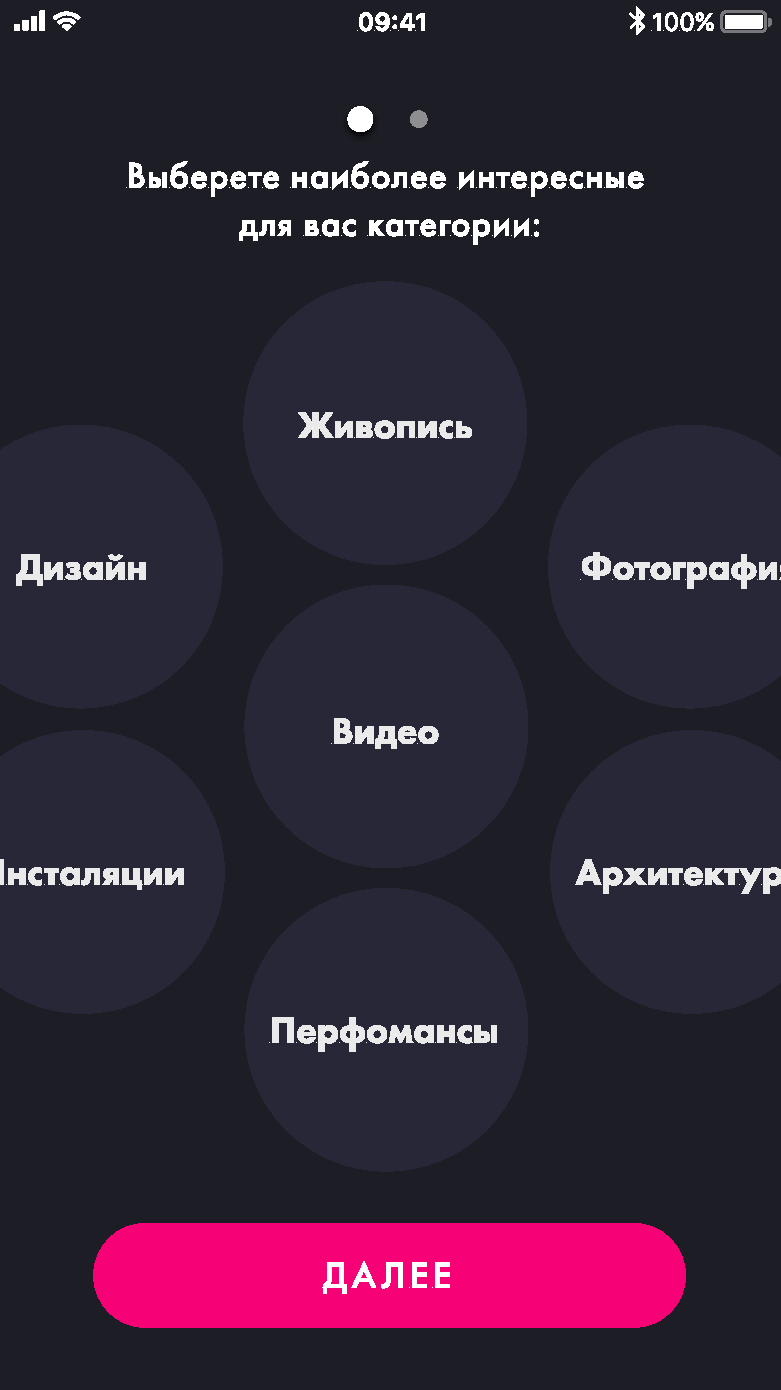
\includegraphics[scale=0.4]{img6}

\end{center}

	\pagestyle{fancy}

\subsection{Статус требований}

\begin{table}[h]
	\caption{Статус требований}
	\centering
	\begin{tabular}{|l|l|}
		\hline
		\textbf{Proposed}    & \begin{tabular}[c]{@{}l@{}}Требование запрошено авторизированным\\ источником.\end{tabular}                                                                                                                                                             \\ \hline
		\textbf{Approved}    & \begin{tabular}[c]{@{}l@{}}Требование проанализировано, его влияние\\ на проект просчитано, и оно было размещено\\ в базовой версии определенной версии.\end{tabular}                                                                                   \\ \hline
		\textbf{Implemented} & \begin{tabular}[c]{@{}l@{}}Код, реализующий требование, разработан,\\ написан и протестирован. Требование отслежено\\ до соответствующих элементов дизайна и кода.\end{tabular}                                                                         \\ \hline
		\textbf{Verified}    & \begin{tabular}[c]{@{}l@{}}Корректное функционирование реализованного\\ требования подтверждено в соответствующем продукте.\\ Требование отслежено до соответствующих\\ вариантов тестирования. Теперь требование\\ считается завершенным.\end{tabular} \\ \hline
		\textbf{Deleted}     & Утвержденное требование удалено из базовой версии.                                                                                                                                                                                                      \\ \hline
		\textbf{Rejected}    & \begin{tabular}[c]{@{}l@{}}Требование предложено, но не запланировано для\\ реализации ни в одной будущих версий.\end{tabular}                                                                                                                          \\ \hline
	\end{tabular}
\end{table}
	\pagestyle{fancy}

\subsection{SWOT-анализ}

\begin{table}[h]
	\centering
	\caption{SWOT-анализ}
	\begin{tabular}{|l|l|}
		\hline
		\textbf{SWOT}                             & \textbf{Арт-квест}                                                                                                             \\ \hline
		\multirow{4}{*}{\textbf{Сильные стороны}} & Наличие топа участников                                                                                                        \\ \cline{2-2} 
		& \begin{tabular}[c]{@{}l@{}}Бонусы и награды за прохождение\\ квестов\end{tabular}                                              \\ \cline{2-2} 
		& \begin{tabular}[c]{@{}l@{}}Возможность отслеживать прогресс\\ определенного участника\end{tabular}                             \\ \cline{2-2} 
		& \begin{tabular}[c]{@{}l@{}}Предоставляет информацию о\\ ближайших выставках\end{tabular}                                       \\ \hline
		\multirow{2}{*}{\textbf{Слабые стороны}}  & Отсутствие сайта                                                                                                               \\ \cline{2-2} 
		& \begin{tabular}[c]{@{}l@{}}Для добавления информации о\\ выставке нужно связываться\\ с разработчиком\end{tabular}             \\ \hline
		\multirow{2}{*}{\textbf{Возможности}}     & \begin{tabular}[c]{@{}l@{}}Привлечь людей к выставкам и\\ показать, что искусство – это интересно\end{tabular}                 \\ \cline{2-2} 
		& \begin{tabular}[c]{@{}l@{}}Разнообразить и улучшить подачу\\ информации, как для подростков,\\ так и для взрослых\end{tabular} \\ \hline
		\textbf{Угрозы}                           & Музеи могут отказаться сотрудничать                                                                                            \\ \hline
	\end{tabular}
\end{table}
	
	\pagestyle{fancy}

\subsection{Список источников}

\begin{enumerate}
	\item[1] ГОСТ 19.101-77 Виды программ и программных документов. //Единая система программной документации. – М.: ИПК Издательство стандартов, 2001.
	\item[2] ГОСТ 19.106-78 Требования к программным документам, выполненным печатным способом. //Единая система программной документации. – М.: ИПК Издательство стандартов, 2001.
	\item[3] ГОСТ 19.301-79 Программа и методика испытаний. Требования к содержанию и оформлению. //Единая система программной документации. – М.: ИПК Издательство стандартов, 2001.
	\item[4] Developer apple. [Электронный ресурс]// URL: https://developers.google.com/ (Дата обращения: 01.12.2019, режим доступа: свободный).
	\item[5] Xamarin documentation. [Электронный ресурс]// URL: https://docs.microsoft.com/en-us/xamarin/ (Дата обращения: 26.11.2019, режим доступа: свободный).
	\item[6] ГОСТ 15150-69 Машины, приборы и другие технические изделия. Исполнения для различных климатических районов. Категории, условия эксплуатации, хранения и транспортирования в части воздействия климатических факторов внешней среды. – М.: Изд-во стандартов, 1997. 
	\item[7] Google developers. [Электронный ресурс]// URL: https://developers.google.com/ (Дата обращения: 02.12.2019, режим доступа: свободный).
	\item[8] ГОСТ 19.602-78 Правила дублирования, учета и хранения программных документов, выполненных печатным способом. //Единая система программной документации. – М.: ИПК Издательство стандартов, 2001.
\end{enumerate}
	
	
	\newgeometry{top=20mm, left=20mm,right=20mm,bottom=0mm}
	\afterpage{\restoregeometry}
	\chead{
	\thepage\\RU.17701729.04.01-01 ТЗ 01-1 ЛУ}

\cfoot{}

\begin{table}[h]
	\begin{tabular}{|c|c|c|c|c|c|c|c|c|c|}
		\hline
		\multicolumn{10}{|c|}{\textbf{Лист регистрации изменений}}                                                                                                                                                                                                                                                                                                                                                                                                  \\ \hline
		\multicolumn{5}{|c|}{Номера листов (страниц)}                                                                                                                                            & \begin{tabular}[c]{@{}c@{}}Всего\\ листов\\ (страниц\\ в\\ докум.)\end{tabular} & \begin{tabular}[c]{@{}c@{}}№\\ документа\end{tabular} & \begin{tabular}[c]{@{}c@{}}Входящий\\ №\\ сопроводит\\ ельного\\ докум. и \\ дата\end{tabular} & Подп. & Дата \\ \hline
		Изм. & \begin{tabular}[c]{@{}c@{}}Изменен\\ ных\end{tabular} & \begin{tabular}[c]{@{}c@{}}Заменен\\ ных\end{tabular} & Новых & \begin{tabular}[c]{@{}c@{}}Аннули\\ рованных\end{tabular} &                                                                                 &                                                       &                                                                                                &       &      \\ \hline
		&                                                       &                                                       &       &                                                           &                                                                                 &                                                       &                                                                                                &       &      \\ \hline
		&                                                       &                                                       &       &                                                           &                                                                                 &                                                       &                                                                                                &       &      \\ \hline
		&                                                       &                                                       &       &                                                           &                                                                                 &                                                       &                                                                                                &       &      \\ \hline
		&                                                       &                                                       &       &                                                           &                                                                                 &                                                       &                                                                                                &       &      \\ \hline
		&                                                       &                                                       &       &                                                           &                                                                                 &                                                       &                                                                                                &       &      \\ \hline
		&                                                       &                                                       &       &                                                           &                                                                                 &                                                       &                                                                                                &       &      \\ \hline
		&                                                       &                                                       &       &                                                           &                                                                                 &                                                       &                                                                                                &       &      \\ \hline
		&                                                       &                                                       &       &                                                           &                                                                                 &                                                       &                                                                                                &       &      \\ \hline
		&                                                       &                                                       &       &                                                           &                                                                                 &                                                       &                                                                                                &       &      \\ \hline
		&                                                       &                                                       &       &                                                           &                                                                                 &                                                       &                                                                                                &       &      \\ \hline
		&                                                       &                                                       &       &                                                           &                                                                                 &                                                       &                                                                                                &       &      \\ \hline
		&                                                       &                                                       &       &                                                           &                                                                                 &                                                       &                                                                                                &       &      \\ \hline
		&                                                       &                                                       &       &                                                           &                                                                                 &                                                       &                                                                                                &       &      \\ \hline
		&                                                       &                                                       &       &                                                           &                                                                                 &                                                       &                                                                                                &       &      \\ \hline
		&                                                       &                                                       &       &                                                           &                                                                                 &                                                       &                                                                                                &       &      \\ \hline
		&                                                       &                                                       &       &                                                           &                                                                                 &                                                       &                                                                                                &       &      \\ \hline
		&                                                       &                                                       &       &                                                           &                                                                                 &                                                       &                                                                                                &       &      \\ \hline
		&                                                       &                                                       &       &                                                           &                                                                                 &                                                       &                                                                                                &       &      \\ \hline
		&                                                       &                                                       &       &                                                           &                                                                                 &                                                       &                                                                                                &       &      \\ \hline
		&                                                       &                                                       &       &                                                           &                                                                                 &                                                       &                                                                                                &       &      \\ \hline
		&                                                       &                                                       &       &                                                           &                                                                                 &                                                       &                                                                                                &       &      \\ \hline
		&                                                       &                                                       &       &                                                           &                                                                                 &                                                       &                                                                                                &       &      \\ \hline
		&                                                       &                                                       &       &                                                           &                                                                                 &                                                       &                                                                                                &       &      \\ \hline
		&                                                       &                                                       &       &                                                           &                                                                                 &                                                       &                                                                                                &       &      \\ \hline
		&                                                       &                                                       &       &                                                           &                                                                                 &                                                       &                                                                                                &       &      \\ \hline
		&                                                       &                                                       &       &                                                           &                                                                                 &                                                       &                                                                                                &       &      \\ \hline
		&                                                       &                                                       &       &                                                           &                                                                                 &                                                       &                                                                                                &       &      \\ \hline
		&                                                       &                                                       &       &                                                           &                                                                                 &                                                       &                                                                                                &       &      \\ \hline
		&                                                       &                                                       &       &                                                           &                                                                                 &                                                       &                                                                                                &       &      \\ \hline
		
	\end{tabular}
\end{table}
\end{document}